\documentclass[11pt]{article}

%
% Packages and settings for mimicking the Jupyter notebook's behavior
%
% \setcounter{secnumdepth}{0} %Suppress section numbers
%\usepackage{parskip} % Stop auto-indenting (to mimic markdown behaviour)
% \usepackage{longtable} % longtable support required by pandoc >1.10
% \usepackage{booktabs}  % table support for pandoc > 1.12.2
% \usepackage[inline]{enumitem} % IRkernel/repr support (it uses the enumerate* environment)
% \usepackage[normalem]{ulem} % ulem is needed to support strikethroughs (\sout)
%								% normalem makes italics be italics, not underlines
%
%

% The hyperref package gives us a pdf with properly built
% internal navigation ('pdf bookmarks' for the table of contents,
% internal cross-reference links, web links for URLs, etc.)
\usepackage{hyperref}
% The default LaTeX title has an obnoxious amount of whitespace. By default,
% titling removes some of it. It also provides customization options.
\usepackage{titling}

% Bibliography 
\usepackage[
	backend=bibtex, % backed bibtex required otherwise it doesn't print anything
	sorting=none %Do not sort at all. All entries are processed in citation order.
]{biblatex}
\addbibresource{references.bib}

\usepackage{geometry} % Used to adjust the document margins
\usepackage{textcomp} % defines textquotesingle

\usepackage{parskip} % omit tab at the beginning of a new paragraph
\usepackage{upquote} % Upright quotes for verbatim code

% For quotes mark
\newcommand{\quotes}[1]{``#1''}

\usepackage[bottom]{footmisc} % enforce footnotes on bottom

\usepackage{comment} % for multilline comments

% Figures and styles
%\usepackage[Export]{adjustbox} % Used to constrain images to a maximum size
\usepackage{float}
%\floatplacement{figure}{H} % forces figures to be placed at the correct location
\usepackage{graphicx} % Basic figure setup
% Required for specifying captions to tables and figures
\usepackage[font=small,labelfont=bf]{caption} 
% subfigures: handle subcaption indexing
\usepackage[subrefformat=parens]{subcaption}
%\usepackage{fancyvrb} % verbatim replacement that allows latex
\usepackage{grffile} % extends the file name processing of package graphics 

% ..to use side captions
\usepackage{sidecap}

% Math
\usepackage{amsmath} % Equations
\usepackage{amssymb} % Equations
\usepackage{amsthm} %  theorems

% Theorems are numbered based on "section", lemmas and corollary based on theorem
\newtheorem{theorem}{Theorem}[section]
\newtheorem{corollary}{Corollary}[theorem]
\newtheorem{lemma}[theorem]{Lemma}

\usepackage{mathrsfs}
% Extended unicode (utf-8) support : ucs incompatible with biblatex!
%\usepackage[mathletters]{ucs}

%% To display conditions/explanation of termns in equations
\usepackage{array}
\newenvironment{conditions}
  {\par\vspace{\abovedisplayskip}\noindent\begin{tabular}{>{$}l<{$} @{${}={}$} l}}
  {\end{tabular}\par\vspace{\belowdisplayskip}}

%%
%% BEGIN DOCUMENT
%%
\begin{document}

\newcommand{\subtitle}[1]{%
  \posttitle{%
    \par\end{center}
    \begin{center}\large#1\end{center}
    \vskip0.5em}%
}

\title{The n x n dots puzzle}
\subtitle{An informal analysis of the classical nine-dots puzzle ``under steroids''}
\date{2020 A.D.}
\author{\\ Andrea Rebolini}

\maketitle

\begin{figure}[H]
\centering

\includegraphics[width=0.4\textwidth]{images/think-out-the-box-icon.jpg}
\end{figure}

\begin{abstract}
The nine-dots puzzle is a mainstream brain-teaser. It's often sponsored by business coaches and management consultants as a benchmark of creative thinking, as its solution requires to ``think outside-the-box".
In the first part of the paper I review the original nine-dots puzzle. I then introduce a generalized version of the original problem, which is extended to an arbitrarily-sized squared grid of points: i.e, the starting \emph{9-dots puzzle} becomes the generic \emph{9-16-25-36..$n\times n$ dots puzzle}. Hence, I present an algorithm to solve the general $n\times n$ puzzle, and also provide a simple proof of optimality of the obtained solutions. Finally, I digress about a possible reformulation of the problem in arithmetical and combinatorial terms.
\\
\\
\textbf{Disclaimer}: the $n\times n$ dots problem has already been solved and treated: references to related works are disclosed all over the paper.
This document simply aims to be a didactic, enjoyable and informal exposition of an appealing mathematical puzzle, whose analysis could be grasped by anyone equipped with a shap mind albeit lacking of a strong mathematical background. Under this premises, I'm pretty confident to say that this is one of the most complete and approachable work on the topic. If you disagree with that and perhaps have suggestions to improve the paper, I am very open to critics and eager to gather feedbacks.
% whether the remarks I make are original or not (I don't want to waste precious days perusing obscure papers and websites for the sole purpose of checking whether some other strange guy in the world rephrased a concept in the same way I did)
\\
\\
\textbf{Keywords}: creative thinking, out-of-the-box thinking, recreational math, nine-dots puzzle, graph theory.

\end{abstract}

\newpage

\hypertarget{nine-dots-puzzle} {
	\section{The nine dots puzzle}
	\label{nine-dots-puzzle}
}
The \textbf{nine-dots puzzle} was first cited by Sam Loyd in his \emph{Cyclopedia of Puzzles}\cite{cyclopedia-puzzle} (see \autoref{fig:egg_puzzle}).
\begin{figure}[H]
	\centering
	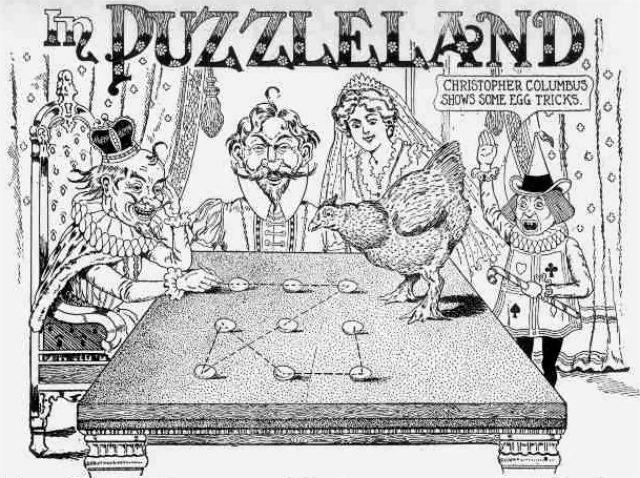
\includegraphics[width=0.54\textwidth]{images/egg_puzzle.jpg}
	\caption{The original illustration of the nine-dots puzzle in the Sam Loyd's "Cyclopedia of puzzles"\cite{cyclopedia-puzzle} (1914). The author entitled it as \emph{the Christoforus Columbus egg puzzle}; this is just a reference to the \emph{egg of Columbus}: you don't actually need 9 eggs to try it yourself.}
\label{fig:egg_puzzle}
\end{figure}
In its basic formulation, the goal is to join nine dots arranged in a squared grid with the minimum number of straight lines, and without lifting the pen. Take your time to figure out the solution...
\begin{figure}[H]
\centering
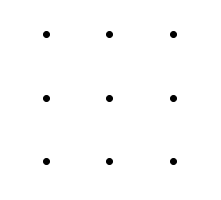
\includegraphics[width=0.3\textwidth]{images/9-dots-grid.png}
\caption{The 9-dots puzzle: join all the points using the fewest possible straight lines, and without lifting the pen.}
\label{fig:9-dots-grid}
\end{figure}
If you concluded that at least five lines are required to join all the points, and your solution looks something like \autoref{fig:9-dots-wrong} alas! You embraced mediocrity and should not complain about your pen-pusher job. But don't worry: contrast your outcome with the king's one in the Sam Loyd's illustration (again \autoref{fig:egg_puzzle}): you're ahead by one line against the king, and thus still highly qualified to rule a nation.
\begin{figure}[H]
\centering
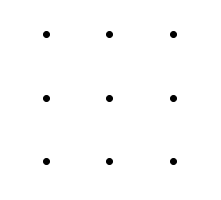
\includegraphics[width=0.3\textwidth]{images/9-dots-grid.png}
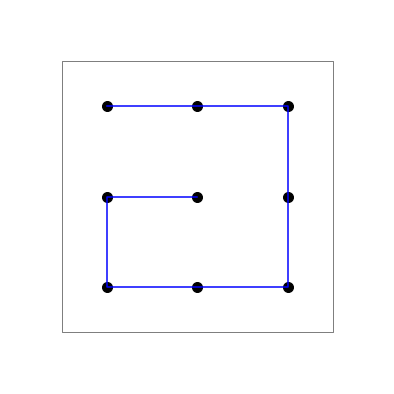
\includegraphics[width=0.3\textwidth]{images/9-dots-wrong-solution.png}
\caption{A suspiciously trivial (and thus wrong) solution to the 9-dots puzzle.}
\label{fig:9-dots-wrong}
\end{figure}
How is it possible to connect the dots with fewer lines?
What hinders most of the people is that they restrict themselves to draw lines within the grid of points, myopically focusing on an immaginary boundary surrounding the grid (similar to the thin grey borders that I maliciously put in the above figures). In order to get to the ``right" solution\footnote{I should say ``to a better attempt": in \hyperlink{appendices}{Appendices}, you'll see why I make such a clarification} you need to \textbf{``think outside the box''}. Using a more creative mindset, a solution can be drawn consisting of just four lines, as shown in \autoref{fig:9-dots-solution}.
\begin{figure}[H]
\centering
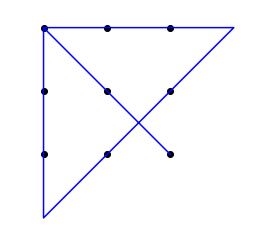
\includegraphics[width=0.3\textwidth]{images/9-dots-solution.png}
\caption{A creative and effective solution to the 9-dots puzzle. Think outside the box!}
\label{fig:9-dots-solution}
\end{figure}
Nice trick, isn't it?! No surprise, this intriguing conundrum was revived by psychologists, salesmen and business coaches, always seeking a nice \emph{coup-de-théâtre} for their demonstrations.


\hypertarget{the-extended-problem} {
	\section{The extended problem}
	\label{the-extended-problem}
}

Since we are now willing to push ourselves ``out of any box", we are now going to consider no less than arbitrarily-sized squared grids: that is, squared grids of $n \times n$ dots ($n >=3$). The goal of the extended puzzle is the same as for the basic version: join all the dots using the fewest possible strokes and without lifting the pen from the paper.\\
If you already struggled with nine dots, don't panic: the generalized problem is easier than it seems. Let's start first with a $4 \times 4$ grid (\autoref{fig:4x4_grid}); don't peek the solution displayed below and take your time to solve...
\begin{figure}[H]
\centering
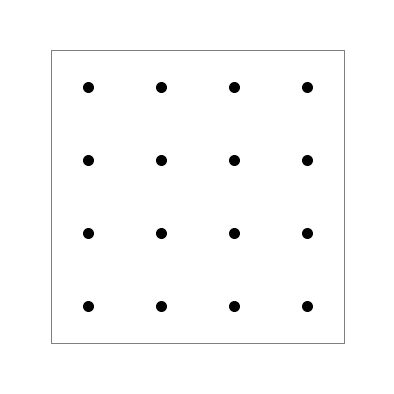
\includegraphics[width=0.3\textwidth]{images/4x4_grid.png}
\caption{Now that you know the trick, you should be able to solve this almost on the fly.}
\label{fig:4x4_grid}
\end{figure}

How many lines did you draw? If you managed to join the dots just with six lines, congratulations! As for the nine-dots puzzle, optimal solutions for this case can only be found by moving outside the box: one possible solution could resemble the guy in \autoref{fig:4x4_grid_solution}.
\begin{figure}[H]
\centering
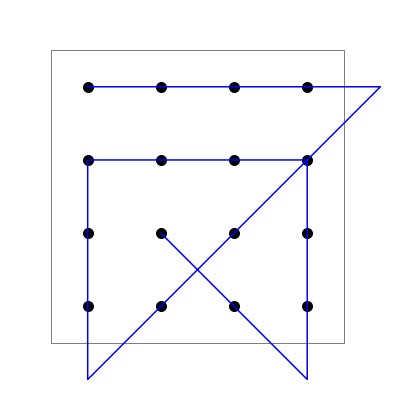
\includegraphics[width=0.3\textwidth]{images/4x4_grid_solution.png}
\caption{A possible out-of-the-box solution to the $4 \times 4$ puzzle.}
\label{fig:4x4_grid_solution}
\end{figure}
However, if you haven't figure it out yet, note that a clever way to solve the $4 \times 4$ grid relies on connecting two adjacent outer borders of the grid and notice that what you are left with is the original nine-dots puzzle (\autoref{fig:4x4_grid_iteration}). Still, six lines have been used.
\begin{figure}[H]
\centering
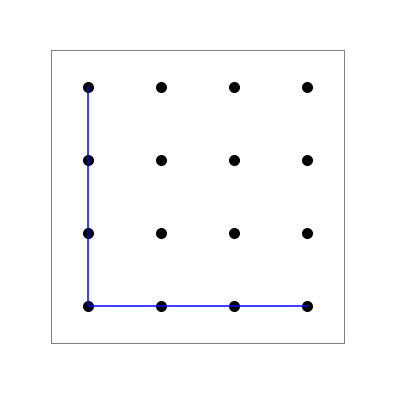
\includegraphics[width=0.3\textwidth]{images/4x4_grid_iteration.png}
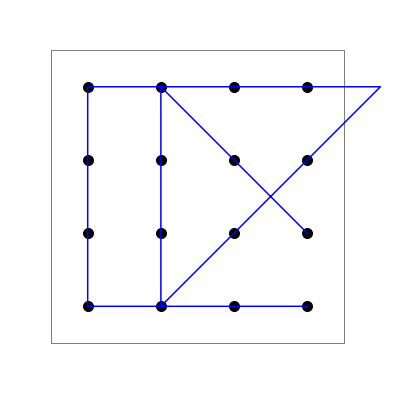
\includegraphics[width=0.3\textwidth]{images/4x4_grid_iteration_solution.png}
\caption{The out-of-the-box solution to the $4\times 4$ grid, leaning on the solution to the original nine-dots puzzle.}
\label{fig:4x4_grid_iteration}
\end{figure}
This clue is actually the keystone to guess the general solution to the problem. If you like challanges, you could exploit the huge hint I just disclosed to figure out the general solution on your own, otherwise keep reading...\\
As you may have already guessed, the general solution can be constructed iteratively. Look again at the solution to the $4x\times 4$ grid in \autoref{fig:4x4_grid_iteration}: each time you connect two adjacent outer borders of the grid you then get an (n-1)-sided grid. It's all downhill from here: in \autoref{fig:6x6_grid_example} you can visualize the recipe to build the general solution applied to a $6\times 6$ grid: first, join two adjacent outer borders so the grid size is reduced by one, then repeat the process as needed, spiraling until you're left with a $3 \times 3$ grid, i.e. the original nine-dots puzzle.
\begin{figure}[H]
\centering
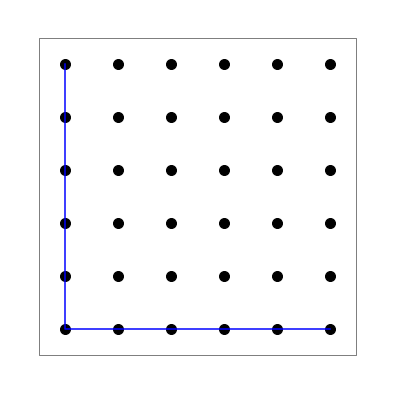
\includegraphics[width=0.23\textwidth]{images/6x6_grid_iteration_01.png}
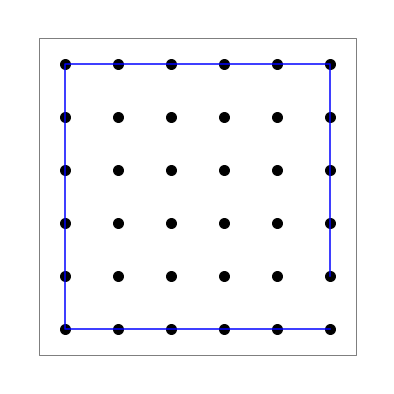
\includegraphics[width=0.23\textwidth]{images/6x6_grid_iteration_02.png}
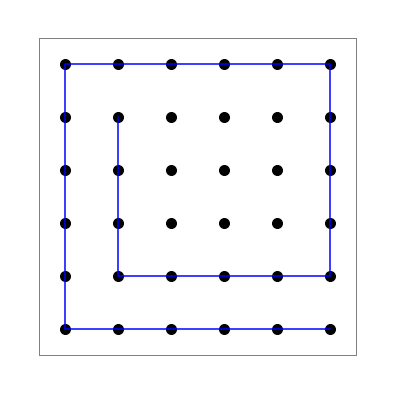
\includegraphics[width=0.23\textwidth]{images/6x6_grid_iteration_03.png}
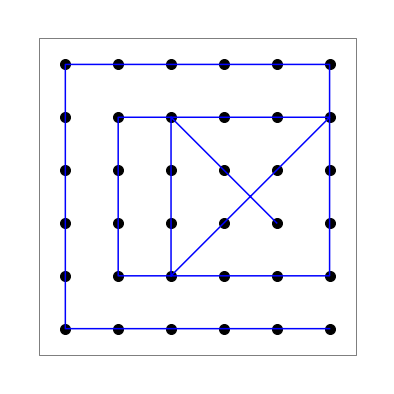
\includegraphics[width=0.23\textwidth]{images/6x6_grid_solution.png}
\caption{The recipe for the general solution, shown on a $6 \times 6$ grid: connect two adjacent outer borders, thus reducing the grid size by one; repeat the process until you are left with the nine-dots puzzle.}
\label{fig:6x6_grid_example}
\end{figure}
Thanks to this recursive argument, we can now state how many lines are at least required to cover an $n \times n$ grid:
\begin{equation}
L_n = 2(n - 1)\ \ \ \  (n >=3)
\label{eqn:line-grid-eq}
\end{equation}
where:
\begin{conditions}
	L_n  &  the number of lines of the optimal solution to the $n\times n$ problem.
\end{conditions}
Indeed, by applying the formula above we get that the optimal solution consists of 4 lines for the $3 \times 3$ grid and of 6 lines for the $4 \times 4$ grid. In \autoref{eqn:line-grid-eq} note how evident the recursive property of the solution is:
\begin{equation}
L_{n} = 2(n-1) = 2(n-2) + 2 = L_{n-1} + 2.\ \ \ \  (n >=3)
\label{eqn:line-grid-eq-recursion}
\end{equation}
In other words, the optimal solution to the $n\times n$ grid consists of two lines (which join two outer borders) plus the number of lines $L_{n-1}$ of the optimal solution to the $(n-1)\times (n-1)$ grid.
Note also that \autoref{eqn:line-grid-eq} does not hold for a $2\times 2$ grid, for which at least three lines are needed to join the dots: damn you Euclid and your in-the-box geometry!

All right, so we finally did it! We found the optimal solution to the squared grid problem! Are you happy with this? ..If you are then I suggest you to always bring a wise friend with you when you have to talk with salespeople or financial advisors, because you are inclined to be fooled by charlatans (such as the author); and the reason is that you should be tormented by this question:\\
\emph{Can we really claim that the solutions output according to the aforementioned recursive recipe are actually optimal and therefore that \autoref{eqn:line-grid-eq} is valid? Isn't that possible (at least for some grid size) to find a clever zig-zagging out-of-the-box polyline consisting of even fewer segments?}\\
Actually, it can be rigorously proved that the minimum number of lines required to solve the $n \times n$ puzzle is given precisely by \autoref{eqn:line-grid-eq}; hence, the spiraling solutions that I depicted above are optimal indeed (I am not that a charlatan after all). The proof can be found in \autoref{proof-extended-solution}: this could turn out to be perhaps a little bit tricky, so feel free to skip it if you are lazy, not curious and unwilling to put a minimal effort to become a better version of yourself.\\
For clarity's sake, I stress that the spiraling solutions (like \autoref{fig:6x6_grid_example}) although elegant and simple, are not the only feasible optimal solutions. As an example, see the weird-looking solution to the $5 \times 5$ grid displayed in \autoref{fig:5x5-grid-weird-solution}: this solution\cite{math-puzzles-site} may not seem as elegant as our spiral polyline, but both the latter and the former count the same number of segments (eight, according to \autoref{eqn:line-grid-eq}) and thus are both optimal.
\begin{figure}[H]
\centering
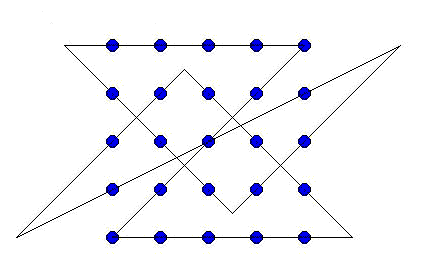
\includegraphics[width=0.3\textwidth]{images/5x5-grid-weird-solution.png}
\caption{This solution to the $5\times 5$ grid\cite{math-puzzles-site} is weird but nonetheless optimal (it counts 8 lines).}
\label{fig:5x5-grid-weird-solution}
\end{figure}
Check out this reference\cite{math-puzzles-site} to peek some other strage optimal solutions. As a nice diversion, you could try to devise bizarre optimal solutions to arbitrary grids without relying on the boring algorithm proposed in this paper.

It's time to conclude this section with a remarkable thought. Take again a closer look at the spiral solution in \autoref{fig:6x6_grid_example}. Wait a minute, what?! Astonishingly, it turns out that for $n >= 5$ the solution can be fully drawn in-the-box! That is, for a grid size of five and upwards, consultants can no longer enthrall us with out-of-the-box tricks.


%% FORMULA
\hypertarget{proof-extended-solution} {
	\subsection{Show me the proof, you cheater!}
	\label{proof-extended-solution}
}

I'm going to prove that in order to cover a $n\times n$ regular grid of points you need at least $2(n - 1)$ segments of a polygonal chain, i.e. lines drawn without lifting the pen from the paper. If you like mathematical hocus-pocus, in this reference\cite{covering-path-paper} is formally proved through a \emph{graph theory} toolkit which is the minimum number of segments of a polygonal chain required to cover a \underline{rectangular $n\times m$ grid}, analysing both cases when crossing of the segments is allowed or not. Of course, such a level of mathematical cleaniness and abstraction would dilute the jocular tone of the paper, therefore I'll restrict myself to a simple geometrical argument\footnote{Psss let's keep it between us, but the author has no other choice, having no proficiency whatsoever in graph theory}. \footnote{After a long search on Internet forums, I actually found out with great disappointment that some other guy already came out with almost the same proof :( \cite{math-stackexchange-squared-grid-proof}.}

First, let's start with the trivial remark that the optimal solution to our $n \times n$ problem could not consist of just horizontal and vertical lines: in this case at least $n + n - 1 = 2n - 1$ segments would be needed to join all the dots, which is more than the lower bound we have found in the previous section (\autoref{eqn:line-grid-eq}). Therefore, we are going to consider covering paths having at least a skew line.\\
Given a polygonal chain spanning an $n\times n$ grid of points, suppose it consists of $L_{h}$ horizontal lines and $L_{v}$ vertical lines (where $L_{h}$, $L_{v} < n$); we can always think to prolong each of this lines so that the whole row or column is covered. Then, by removing all these rows and columns we are left with a $(n - L_{h}) \times (n - L_{v})$ grid: this grid may not be regular nor squared but the following considerations still apply.\\
So, let's deal with the residual $(n - L_{h}) \times (n - L_{v}$) grid: we've already run out of horizonal and vertical lines, therefore we are allowed to join the dots just with skew lines. Focus in particular on the outer borders of the grid: these count $2(N-L_{h}$) + $2(N - L_{v})$ - 4 dots, and we have to reach them all with skew segments; since at most two dots of the borders could be joined with diagonals, at least the following number of segments is needed:
\begin{equation}
L_{s}^{LB} \equiv (2(n-L_{h}) + 2(n - L_{v}) - 4) / 2 = (n- L_{h}) + (n - L_{v}) - 2
\label{eqn:skew-lower-bound}
\end{equation}
where $L_{s}^{LB}$ stands for the lower bound on skew lines.\\
Can I have some drum-roll please? To summarize, we imagined a generic solution using $L_{h}$ horizonal and $L_{v}$ vertical lines, then we have found the lower bound on the number of skew lines (\autoref{eqn:skew-lower-bound}). Thus, we can state that to cover $n\times n$ dots with a polygonal chain we need at least this number of lines:
\begin{equation}
L_{h} + L_{v} + L_{s}^{LB} = L_{h} + L_{v} + (n - L_{h}) + (n - L_{v}) - 2 = 2n - 2 = 2(n-1)
\label{eqn:lower-bound-grid}
\end{equation}
Exactly the result claimed in \autoref{eqn:line-grid-eq}! Clean the sweat on your forehead, pull back your jaw and enjoy. 

%% BEGIN COMMENT
%% Lemma for a trivial lower bound, probably obsolete now that we gave the proof of optimality
\begin{comment}
After all, the only trivial lower bound that we can state is the following:
\begin{lemma}
At least N+1 lines are required to optimally solve the squared grid problem for a $N\times N$ grid; i.e. N+1 is a lower bound on the number of lines of the optimal solution.
\label{lemma:lower-bound}
\end{lemma}
\begin{proof}
Indeed, we have to draw at least N+1 straight lines to join all the dots on a N-sided grid even without being constrained to hold the pen on the paper. That is, the optimal solution to the \underline{unconstrained} problem requires N+1 strokes, therefore the solution to the constrained problem we are considering cannot be cheaper. You could exploit \autoref{fig:unconstrained_solution} to grap this.
\end{proof}
According to the lemma, for a 4x4 grid the lower bound on the number of lines of the optimal solution is five\footnote{Btw, the lemma certifies instead why four lines are the optimum in the original nine-dots puzzle} and not six. 
A rigorous and non-constructive proof that the lower bound for our problem is actually larger relies ultimately on the optimal way to partition a set under some constraint\footnote{in our case the constraints are those imposed by the geometric arrangment of the dots and that we are not allowed to lift the pen from the paper}: I would gently return to this topic in \autoref{arithmetical-interpretation}, in which I play with numbers and digress on the arithmetical interpretation of the solution to the squared grid puzzle. Anyway, the full mathematical analysis would be quite complicated. 
\begin{figure}[H]
\centering
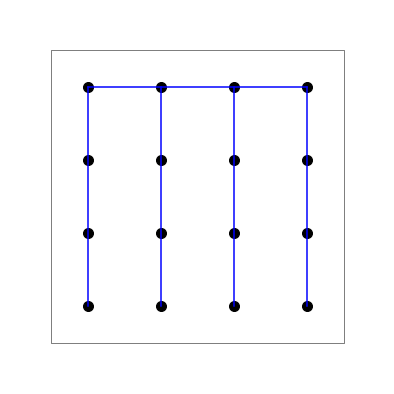
\includegraphics[width=0.3\textwidth]{images/unconstrained_solution_4x4.png}
\caption{An optimal solution to the \underline{unconstrained} problem (you are allowed to lift the pen from the paper) shown on a 4x4 grid. The solution to our problem must have at least the same number of lines.}
\label{fig:unconstrained_solution}
\end{figure} 
Thus, only by examining the form of the trials and exploiting the geometry of the grid we can state that a solution with five lines is not actually feasible; and consequently that our solutions consisting of six lines are actually optimal ones.
\end{comment}
%% END COMMENT

\hypertarget{arithmetical-interpretation} {
	\subsection{An arithmetical interpretation of the puzzle}
	\label{arithmetical-interpretation}
}
I know that at first glance you find geometric figures more relaxing and appealing than formulas or numbers, despite your level of mathematical sophistication; and that's fine: after all, I guess my reader is a mammal and therefore endowed with a powerful visual cortex refined by ages of evolution. Even the ancient Greeks, the mathematical nerds \emph{par excellence} of the ancient world, concieved their results through the inspection of geometrical entities. Pythagoras would have never codified the idea of \quotes{three} into a single doubly-bulged symbol like the arab \quotes{3}: he and his followers would have probably pictured a triangle or perhaps three dots arranged on the vertices of a triangle.\\
Our puzzle is gloriously geometrical in nature and would have probably been a greatest hit among the ancient Greeks. Nonetheless, since the connection between geometry and arithmetic could sometimes be very profound and illuminating\footnote{I hope my reader is not one of those obsessive weirdos seeking everywhere for the Fibonacci sequence or the Golden ratio.}, let's try to rephrase our squared grid problem in arithmetical terms and see if something interesting comes out.

The basic idea is quite simple: we have an $n\times n$ squared grid of dots, which represent the squared integer $n^{2} (n \in \mathbb{N})$; joining all the points with segments corresponds to summing the numbers of points belonging to each segment in order to get the value $n^2$; if one point is touched by more than one segment is anyway counted only once. See \autoref{fig:grid-arithmetical-interpretation} for a visual example.
\begin{figure}[H]
\centering
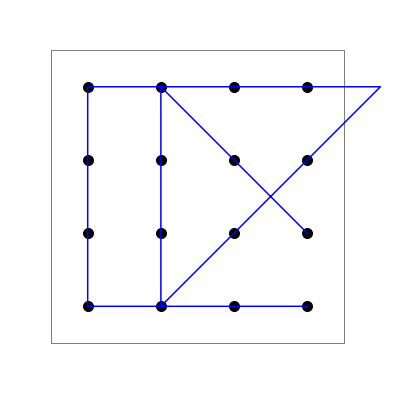
\includegraphics[width=0.25\textwidth]{images/4x4_grid_iteration_solution.png}
\caption*{\emph{16 = 4 + 3 + 3 + 2 + 2 + 2}}
\caption{A possible arithmetical interpretation of a grid covering path: the numbers of points falling on each segment are summed in order to get the squared integer associated to the grid, in this case $4\times 4=16$. Each point must be counted only once even if it belongs to multiple lines. I arbitrarily decided the grouping/counting order to be the encounter order of the lines as drawn by means of the recipe depicted in \autoref{fig:6x6_grid_example}.}
\label{fig:grid-arithmetical-interpretation}
\end{figure}

Under this light, the squared grid puzzle (which -recall- requests to connect all the dots of the grid with the fewest number of strokes and without lifting the pen from the table) might be formulated as a problem of combinatorics:\\
\\
\emph{
For each squared integer $n^2$, consider all the possible ways to sum integers to get that number. The goal is to find the shortest sequences of integers summing to the given squared integer $n^2$ and satisfying the constraints inherited from the geometrical problem:
\begin{itemize}
	\item
		Each line of the solution could span at most n points $\iff$ Each addend must be less than or equal to n.
	\item
		The segments are drawn without lifting the pen from the paper $\iff$ I really don't have any clue on how to codify this in arithmetical terms!
\end{itemize}
}
Yes, shame on me! I did not even figure out how to rephrase the puzzle in a combinatorial fashion: this is perhaps an interesting open point of the paper, and so far I didn't found any related literature on it. The combinatorial counterpart of the squared grid puzzle seems in any case quite complicated stuff, and could probably be ascribed to the fascinating field of mathematics known as combinatorial geometry\cite{wolfram-combinatorial-geometry}.

Having shown off my limits, I restrict the reach of this section to discuss the arithmetical interpretation of the spiral-shaped solution introduced in the previous sections. The solutions to the lowest-order grids are displayed in \autoref{fig:solution-number-decomposition} together with the decomposition of the squared integer $n^2$ the solution represents.
\begin{figure}
\begin{subfigure}[b]{.3\linewidth}
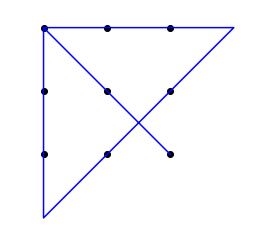
\includegraphics[width=\linewidth]{images/9-dots-solution.png}
\caption{9 = 3+2+2+2}\label{fig-a}
\end{subfigure}
\hfill
\begin{subfigure}[b]{.3\linewidth}
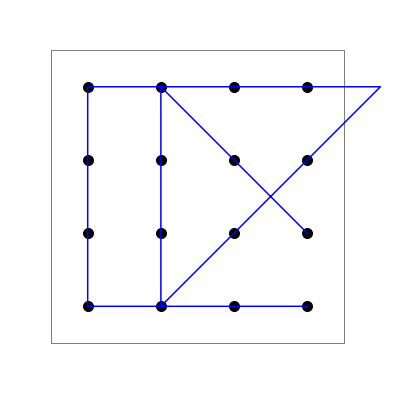
\includegraphics[width=\linewidth]{images/4x4_grid_iteration_solution.png}
\caption{16=4+3+3+2+2+2}\label{fig-b}
\end{subfigure}
\hfill
\begin{subfigure}[b]{.3\linewidth}
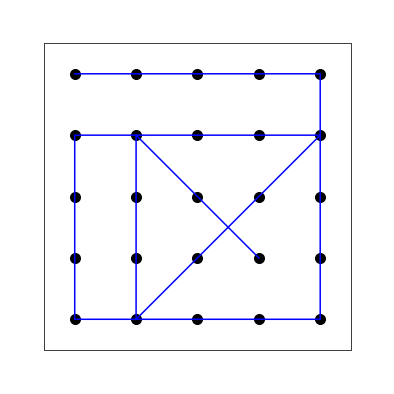
\includegraphics[width=\linewidth]{images/5x5-grid-solution.png}
\caption{25=5+4+4+3+3+2+2+2}\label{fig-c}
\end{subfigure}
\hfill
%% BEGIN COMMENT
\begin{comment}
\begin{subfigure}[b]{.23\linewidth}
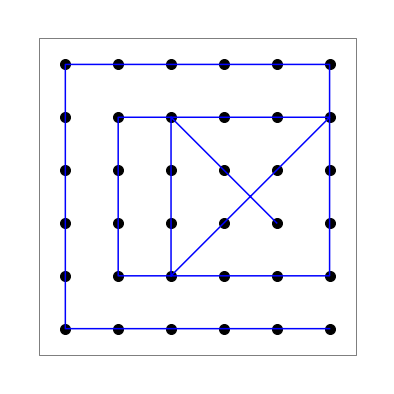
\includegraphics[width=\linewidth]{images/6x6_grid_solution.png}
\caption{36=6+5+5+4+4+3+3+2+2+2}\label{fig-d}
\end{subfigure}
\end{comment}
%% END COMMENT
\caption{The spiral-shaped solutions to the puzzle for the lowest-order grids, together with the related arithmetical decomposition of the squared integer.}
\label{fig:solution-number-decomposition}
\end{figure}
So, using a consistent counting convention we can see a recursive relationship:\\
\begin{enumerate}
	\item[] % [] suppress bullet
		$3 \times 3 = 9 \Leftrightarrow 3 + 2 + 2 + 2 \equiv S(3)$
	\item[]
		$4 \times 4 =16 \Leftrightarrow 4 + 3+ 3 + 2 + 2 + 2 \equiv S(4) = 4 + 3 + S(3) $
	\item[]
		$5 \times 5 =25 \Leftrightarrow 5 + 4 + 4 + 3+ 3 + 2 + 2 + 2 \equiv S(5) = 5 + 4 + S(4)$
\end{enumerate}
and so on and so forth, where I used the notation $S(n)$ to indicate the chosen sum decomposition of the squared integer. This progression can be summarized as follows:
\begin{equation}
\begin{aligned}
&S(n) = n + n -1 + S(n - 1), \ \ \ \ \ \  (n \geq 3, n \in \mathbb{N})\\
&S(3) = 3 + 2 + 2 + 2
\end{aligned}
\end{equation}
which in turn is a convoluted way to represent the decomposition:
\begin{equation}
n^2 = n + n - 1 + n - 1 + n - 2 + .. + 3 + 2 + 2 + 2.
\end{equation}
I know what you're thinking: all these arithmetical manipulations seem pretty pointless, and you are right! My goal in this section was just to shed light on a potential interesting branch the analysis of the puzzle could lead to; if that makes sense, you could try tinkering with this idea on your own and let us know the results.

\hypertarget{final-notes}{
	\section{Final notes}
	\label{final-notes}
}

\paragraph{Acknowledgements} \mbox{} \\ % mbox needed for having carriage return after "paragraph"
Marco Ripà posed the squared grid brain-teaser during one of his stimulating YouTube live sessions (in Italian)\cite{marco-ripà-yt}: that's how this problem came to my attention; I am obliged to him for the great fun I had in tackling this problem, which in turn inspired all the analysis and ideas that followed. Marco Ripà himself published many papers on the extension of the \emph{nine-dots puzzle} to arbitrarily-sized grids and to multiple dimensions!\cite{ripà-paper-nxnxn-extension, ripà-paper-nxnxn-extension-02, ripà-paper-nxnxn-extension-03}

\paragraph{Technical note for computer nerds} \mbox{} \\
Python was used to code the solver algorithm and produce the explanatory images of the paper. You can find the implementation in the attached Jupyter notebook, in which you can also display a nice animation drawing the solution to the puzzle.

\paragraph{Future developments} \mbox{} \\
I'll address the problem in multiple dimensions, you bet! I would also like to extend the solver's code to handle this more general case; hence, as a plus I could produce animations drawing the solution for three-dimensional grids. The attemp to rephrase the puzzle as a problem of combinatorics, discussed in \autoref{arithmetical-interpretation}, led to a \emph{cul-de-sac}: but who knows, right?\\
In this reference\cite{math-puzzles-site} the dots of the grid are joined through arc of circumferences instead of lines: that seems a quite funny variation!\\
It would also be possible to analyze our puzzle with the additional constraint that the segments of the polyline are not allowed to cross each other. Beware: the more general and sophisticad the problem becomes, the more likely we'll be forced to study \emph{graph theory}!

Of course, you and I can keep going to add proposals into the suggestion box: anyway, recall that the only thing that matters is not to put ourselves into it.

%% APPENDICES %%
\hypertarget{appendices}{
	\section{Appendices}
	\label{appendices}
}

\hypertarget{best-solutions-nine-dots-puzzle} {
	\subsection{Best solutions to the nine-dots puzzle}
	\label{best-solutions-nine-dots-puzzle}
}

\vspace{1cm}

% side caption [width][positioning]
\begin{SCfigure}[1.5][!h]
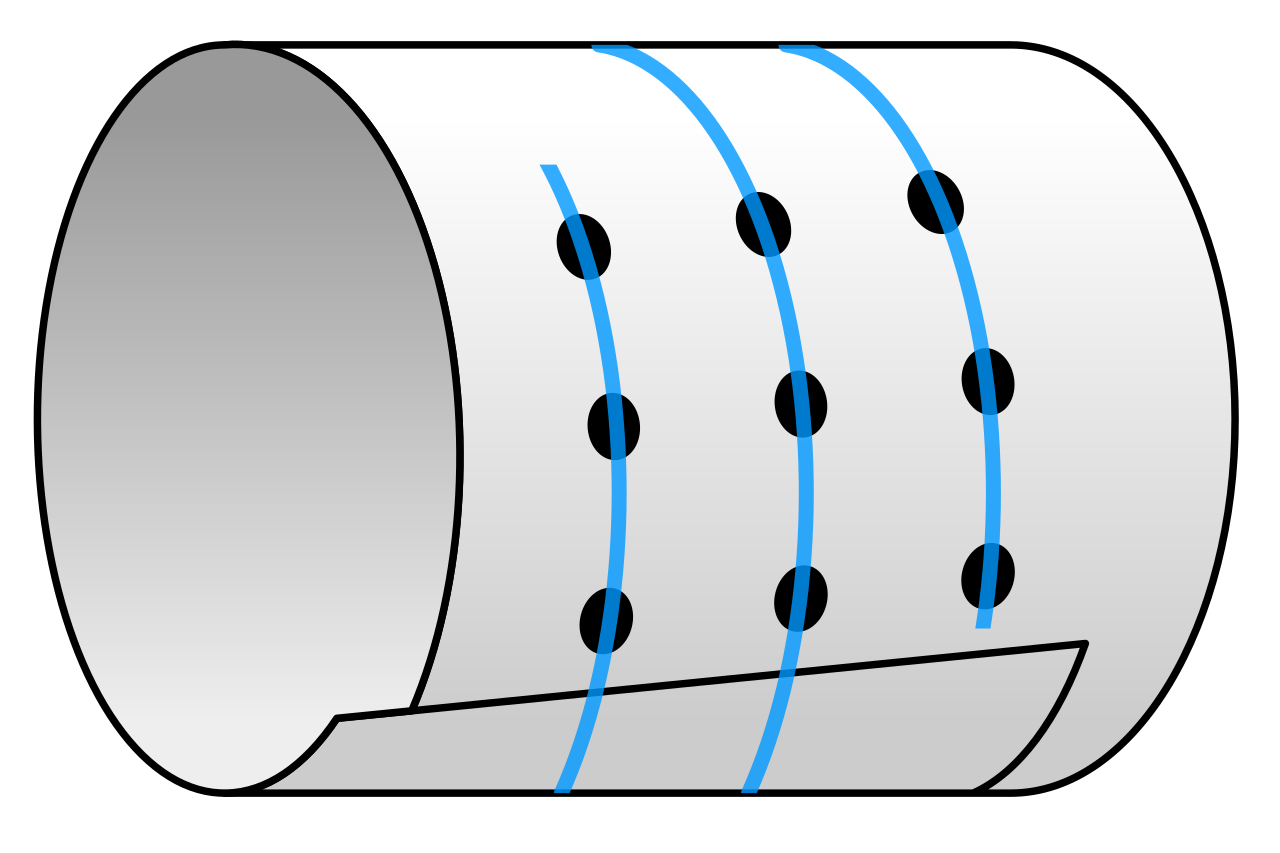
\includegraphics[width=0.35\textwidth]{images/nine-dots-roll-paper.png}
\caption{You can roll the paper and join the dots with a single line\cite{wikipedia-out-of-the-box}.}
\label{nine-dots-roll-paper}
\end{SCfigure}

\begin{SCfigure}[1.5][!h]
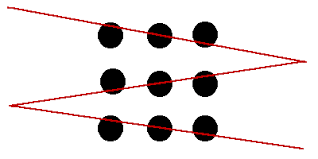
\includegraphics[width=0.35\textwidth]{images/nine-dots-finite-width.png}
\caption{Cheat on the size of the dots: the puzzle should specify whether the dots are physical or geometrical. Question: given a dot size, which is the smallest piece of paper allowing you to still solve the puzzle using this trick?}
\label{nine-dots-dots-width}
\end{SCfigure}

\begin{SCfigure}[1.5][!h]
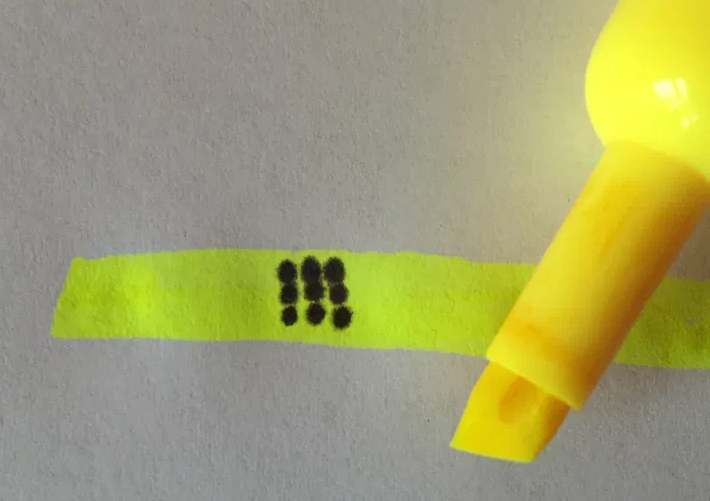
\includegraphics[width=0.3\textwidth]{images/9-dots-line-width.png}
\caption{Cheat on the size of the lines (source: Google images..).}
\label{nine-dots-line-width}
\end{SCfigure}

\begin{SCfigure}[1.5][!h]
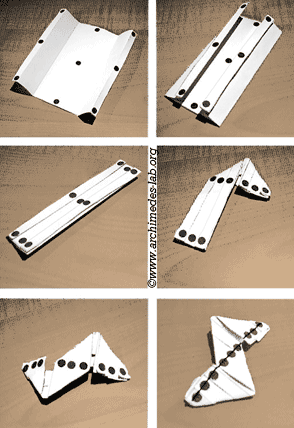
\includegraphics[width=0.3\textwidth]{images/9-dots-origami-solution.png}
\caption{A one-line origami solution (source: www.archimedes-lab.com).}
\label{nine-dots-origami-solution}
\end{SCfigure}

You can also cut the paper in stripes each one containing a row of three dots, line these stripes and finally draw a single segment through them...Do you have some other ace up the sleeve?

\hypertarget{appendices-in-the-box} {
	\subsection{Legitimate in-the-box}
	\label{appendices-in-the-box}
}
\begin{figure}[H]
\centering
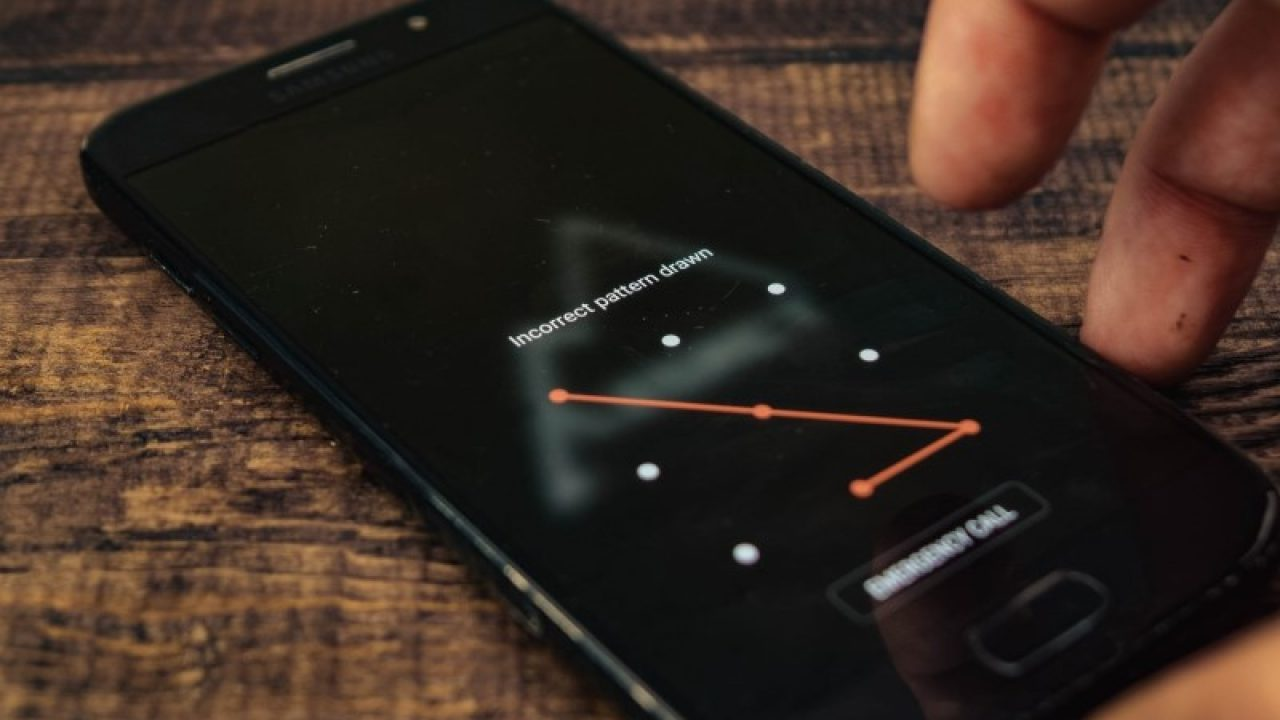
\includegraphics[width=0.5\textwidth]{images/smartphone_nine_dots.jpg}
\caption{Now you'll see the nine-dots puzzle everywhere! NB: even your smartphone enforces you to draw patterns inside-the-box. (source: Google images..)}
\label{smartphone-nine-dots}
\end{figure}

\begin{figure}[H]
	\centering
	\begin{subfigure}[b]{0.32\textwidth}
	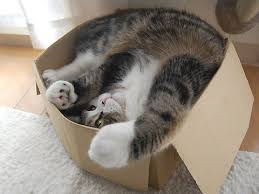
\includegraphics[width=\textwidth]{images/cat-in-the-box-1.jpg}
	\end{subfigure}
	\hfill
	\begin{subfigure}[b]{0.32\textwidth}
	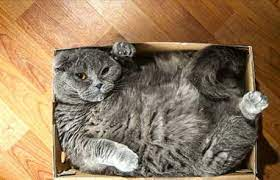
\includegraphics[width=\textwidth]{images/cat-in-the-box-3.jpg}
	\end{subfigure}
	\hfill
	\begin{subfigure}[b]{0.32\textwidth}
	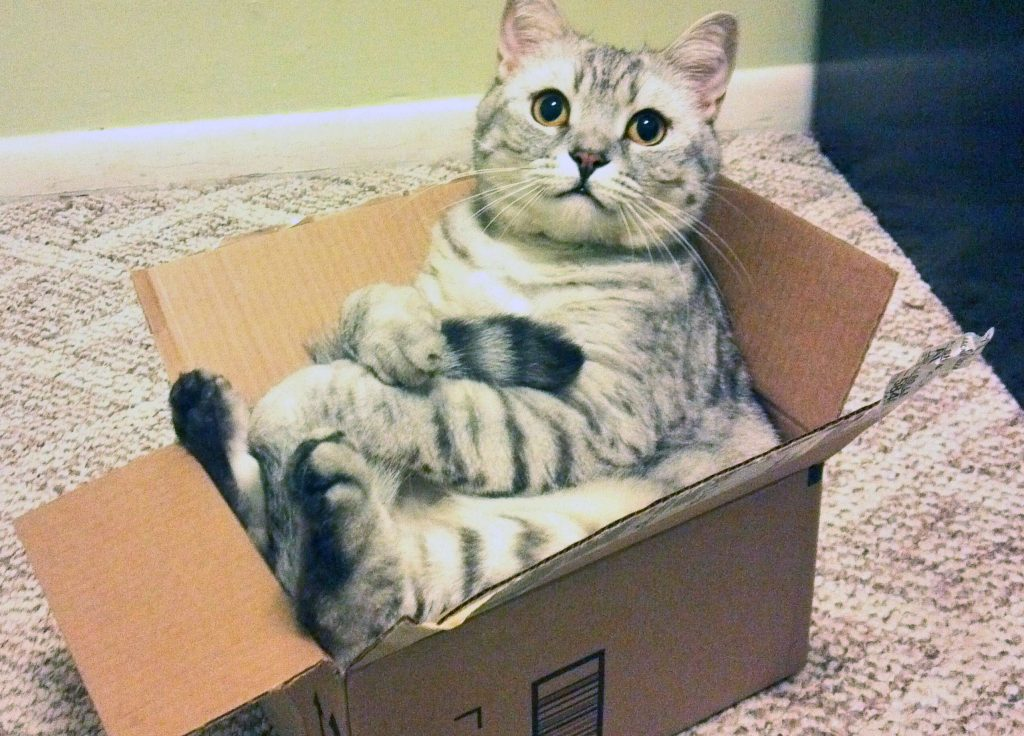
\includegraphics[width=\textwidth]{images/cat-in-the-box-4.jpg}
	\end{subfigure}
	\caption{Awww.. they are allowed to stay in-the-box. (source: Google images..)}
	\label{fig:cat-in-the-box}
\end{figure}


%% REFERENCES %%

%% if using biblatex
\printbibliography[heading=bibintoc] % heading -> add bibliography to the table of contets

\end{document}
